\documentclass[12pt]{article}

\usepackage[margin=2cm]{geometry}
\usepackage{indentfirst}
\usepackage[pdftex,colorlinks,linkcolor=black,urlcolor=blue]{hyperref}
\usepackage{afterpage}
\usepackage[pdftex]{graphicx}
\usepackage{alltt}
\usepackage{array}
\usepackage{setspace}

\newcommand{\jump}{~\newline}
\newcommand{\replica}[1]{\textsf{#1}}
\newcommand{\krusader}{\textsf{KRUSADER}~}
\renewcommand{\url}[1]{\href{#1}{\texttt{#1}}}
\renewcommand{\baselinestretch}{1.08}
\renewcommand{\arraystretch}{1.2}

\newcommand{\tighter}
{ 
	\setlength{\itemsep}{-1mm}
	\setlength{\parsep}{-1mm}
} 

%\setlength{\extrarowheight}{2mm}

\begin{document}

\title{User Manual \\ for \\ {~} \\ \Huge \krusader \normalsize \\ {~} \\
\textit{Ken's Rather Useless Symbolic Assembly Development Environment for the Replica 1}\\
or is that \textit{Reasonably Useful?}  You decide!}

\author{Ken Wessen \\ \texttt{ken.wessen@gmail.com} }
\date{Version 1.3 -- \today}
\maketitle

\section{Introduction}

\krusader is a program written to allow assembly language development on the Replica 1 -- an Apple 1 clone designed by Vince Briel\footnote{\url{http://www.brielcomputers.com}}, and described in the book \textit{Apple 1 Replica Creation: Back to the Garage} by Tom Owad\footnote{\url{http://www.applefritter.com/replica}}.
\krusader includes a simple shell and editor, a single-pass symbolic assembler, and a disassembler, and fits in just under 4K (so it is
small enough to fit in the 8K of Replica 1 ROM along with the monitor and Apple BASIC).  
Although designed for the Replica 1/Apple 1, there is very little system dependent code, and since full source code is provided, \krusader can easily be adapted to any other 6502 based system.  However, it's limitations may mean it is not an appropriate tool in many cases (for example, it has no concept of a file-system and so would not be particularly suitable for use on an Apple II).

\krusader handles a fairly standard and expressive syntax for its assembly source code.  
For users who are unfamiliar with the 6502 instruction set, I recommend the introduction by Andrew John Jacobs that can be found at \url{http://www.obelisk.demon.co.uk/6502/} (and the associated \url{http://www.obelisk.demon.co.uk/65C02/}).  
On a Replica 1, \krusader can assemble over 200 lines of code per second, and given its 32K of RAM, the defaults provide space for around 20K of tokenised source code, 7K of generated code, and up to 256 global symbols.

The \krusader distribution is comprised of source files for various versions (the differences between these versions is described in section \ref{sec:history}), and two binaries for the latest version -- one to be loaded in high RAM at addresses \$7100-\$7FFF, and the other that belongs in ROM from \$F000-\$FEFF.  Since source is provided, alternative binaries are easy to produce.  I use the 6502 simulator by Michal Kowalski\footnote{\url{http://home.pacbell.net/michal\_k/}} to assemble the object code, and test it on the Pom1 simulator\footnote{The original is at \url{http://www.chez.com/apple1/Apple1project/}, and the version at \url{http://school.anhb.uwa.edu.au/personalpages/kwessen/apple1} fixes various bugs, and adds the capability to emulate a 65C02-based Replica 1.} and my Replica 1.  Although the latest version of \krusader supports the 65C02, it contains only 6502 code itself, and this manual will cover the 6502 features first, saving a discussion of the 65C02 enhancements until section \ref{sec:65C02}.  Addresses quoted in this manual will be for the high RAM version of the code, with the ROM version values following in brackets, but these values are easily offset for a version with any particular starting address.

\section{Sample Session}
\label{sec:samplesession}

The best way to give a quick overview of the system and its operation is to work through a couple of simple examples.  First thing is to load the program, and once loaded run it by typing \texttt{7100R}(\texttt{F000R}).  At this point you will be presented with a brief message showing the version of the assembler you are running, followed by the shell prompt \replica{?~}.  Type \replica{N} to enter a new program, and enter the code shown below.  The column layout is important, with the source organised in \emph{fields}.  After the current line number is printed by the editor, the next 6 characters are the \emph{label field}, then after a space there is the 3 character \emph{mnemonic field}, then after a space a 14 character \emph{arguments field}, and finally a \emph{comments field} of maximum 10 characters.
Hitting tab or space will automatically progress you to the next field, and to finish entering code, hit the escape key (hit return first though, or you will lose the current line).  If you make an error typing a line, hitting backspace will return you to the start of the line (there is no true backspace on the Apple 1, and I have chosen not to implement the underscore-as-backspace hack used in the Apple 1 monitor and Apple 1 BASIC since it confuses the syntactically important column layout).  If you only notice an error after hitting return and need to change a line, type \replica{E nnn}, where \replica{nnn} is the line number in question (it is not necessary to enter any leading zeroes).  If you missed a line out altogether, type \replica{I nnn} to insert at line \replica{nnn}.
\begin{alltt}
? N
000        LDA #'A'
001 LOOP   JSR $FFEF
002        CLC
003        ADC #$1
004        CMP #'Z'+1
005        BNE LOOP
006        RTS
007<esc>
\end{alltt}
When you have finished entering the source, type \replica{L} to list the code, and then \replica{A} to assemble it.  You should see the assembler output \texttt{0300-030C}, indicating the target memory locations used by the assembled code.  Any errors detected in the code will be displayed at this point, and can be fixed using either the \replica{I} and \replica{E} commands described above, or the \replica{X nnn mmm} command for deleting a range of lines (the second argument \replica{mmm} is optional).  Once the code has been successfully assembled, run it by typing \replica{R \$300}.  The program will run and output the string \begin{alltt}ABCDEFGHIJKLMNOPQRSTUVWXYZ\end{alltt} and then return to the shell (because of the final \texttt{RTS}).

In order to illustrate some more advanced features of the assembler, a second, more complicated example is the following.
\begin{alltt}
000 ECHO   .=  $FFEF
001 START  .=  'A'
002 END    .=  'Z'
003 STEP   .=  $30
004 
005 SETUP  .M  $280
006        LDA #$1
007        STA STEP
008        LDA #START
009        RTS
00A 
00B FWD    .M  $300
00C .LOOP  JSR ECHO
00D        CLC
00E        ADC STEP
00F        CMP #END
010        BMI .LOOP
011        RTS
012
013 BACK   .M  $320
014 .LOOP  JSR ECHO
015        SEC
016        SBC STEP
017        CMP #START
018        BPL .LOOP
019        RTS
01A
01B MAIN   .M  $340
01C        JSR SETUP
01D        JSR FWD
01E        JSR BACK
01F        RTS
\end{alltt}
Again, type \replica{L} to list the code.
Since this program is longer than 24 lines (i.e.~one Apple 1 screen), the listing will pause after 22 lines and wait for a keypress.  
Hitting return will move the listing forward by one line, escape will cancel the listing, and any other
key will list the next 22 lines.  Typing \replica{A} will assemble the code -- this time made up of 4 modules,
each with their own starting address.  The assembler will output the following upon successful assembly:
\begin{alltt}
? A
0300-02FF
SETUP  005 0280-0286
FWD    00B 0300-030A
BACK   013 0320-032A
MAIN   01B 0340-0349
?
\end{alltt}
This output shows the first source line number and the memory locations used by each module in the source code (the first line can be ignored because no code is generated prior to the declaration of the \texttt{SETUP} module).
Hitting \replica{M} will show the memory taken up by the source code, in this case \texttt{2000-20E5}(\texttt{2300-23E5}), 
and the value of global symbols can be queried by using the \replica{V} command -- e.g.~typing 
\replica{V MAIN} will get the response \texttt{0340}.  This is important, because it is the entry
point for this program, and running it by typing either \replica{R \$340} or \replica{R MAIN} will result in the output:
\begin{alltt}
ABCDEFGHIJKLMNOPQRSTUVWXYZYXWVUTSRQPONML
KJIHGFEDCBA
\end{alltt}

Some other relevant features of this second example are the use of blank lines for layout, and symbols to represent both constants 
(e.g.~\texttt{START  .=  'A'}) and memory locations (e.g.~\texttt{STEP   .=  \$30}).
Also note the use of the \emph{local label} \texttt{.LOOP} in both the \texttt{FWD} and \texttt{BACK} modules.
Local labels are indicated by an initial '\texttt{.}', and have module level scope only.
The \texttt{.=} and \texttt{.M} commands are two directives recognised by the assembler for
defining symbols and modules respectively.  It is not necessary to give a memory location
argument to the \texttt{.M} directive, and indeed only in very special circumstances would you wish to do so.

\section{Shell Commands}

The previous section introduced most of the available shell commands, in the context of a sample interactive session.
Shell commands are entered in response to the \replica{?} prompt, and are all single key commands, with between zero and two arguments.  If the shell cannot process an entered command, \texttt{ERR: SYN} is output to indicate a syntax error.  Five of the twelve shell commands are for source editing, and the others are for assembling, running, disassembling, querying symbols and source memory, entering the monitor, and recovery.
Table \ref{tab:shellcmds} gives a summary of all commands and their syntax.
\begin{table}[p]
	\centering
	\begin{tabular}{|c|c|p{10cm}|} \hline
	\textbf{Command} & \textbf{Arguments} & \textbf{Action} \tabularnewline
	\hline
	\replica{N} & & Start a new program.  This command will
									clear any existing source, and prompt
									for source entry from line 000.\tabularnewline
	\replica{I} & $<$\replica{nnn}$>$ & Insert code from line \replica{nnn}, or at
									the end if no argument.  If $k$ lines are inserted, existing
									lines from \replica{nnn} are shifted down by $k$.\tabularnewline
	\replica{L} & $<$\replica{nnn}$>$ & List the source starting from line
									\replica{nnn}, or the beginning if no argument.  The 
									listing pauses for input every page -- hitting return shows the next
									line, escape cancels the listing, and any other key shows
									the next page.\tabularnewline
	\replica{X} & \replica{nnn~}$<$\replica{mmm}$>$ & Delete from lines
									\replica{nnn} to \replica{mmm} inclusive.  If just one
									argument, delete line \replica{nnn} only.  Care must be taken
									since this will change the line number associated with all
									subsequent source lines.  Delete cannot be undone.\tabularnewline
	\replica{E} & \replica{nnn} & Edit line \replica{nnn}, and insert after.
									This is equivalent to typing \replica{X nnn} followed by
									\replica{I nnn}, so the existing line is deleted
									immediately, and as for the \replica{X} command, it
									cannot be recovered.\tabularnewline
	\replica{M} & & Show the memory range used to store the current source 
									code.\tabularnewline
	\replica{A} & & Assemble the current source code.\tabularnewline
	\replica{V} & \replica{LABEL} & Show the value of the given label.\tabularnewline
	\replica{R} & \replica{\$nnnn} or \replica{LABEL} & 
									Run from address \replica{\$nnnn}.  If the
									program ends with an RTS, control is returned to the
									shell.  Otherwise, re-enter the shell at address
									\texttt{\$711A}(\texttt{\$F01A}).\tabularnewline
	\replica{D} & $<$\replica{\$nnnn} or \replica{LABEL}$>$ & Disassemble 20 instructions
									from address \replica{\$nnnn}, or continue from the last
									address if no argument.\tabularnewline
	\replica{\$} & & Drop into the Apple 1 Monitor.  You can re-enter the shell at address
									\texttt{\$711A}(\texttt{\$F01A}).\tabularnewline
	\replica{P} & \replica{$<$c$>$} & Panic!  This command attempts to recover lost source
									(usually due to zero page data corruption).  If the 1st
									line of source starts with a label, then give the first
									letter of that label as an argument to this command.  For
									more detail, see the section on source tokenisation
									\ref{sec:token}\tabularnewline
	\hline
	\end{tabular}
	\caption{\krusader shell commands.  Note that any shell commands that use labels
	are dependent on the assembler's global symbol table being intact, specifically the pointer information
	in zero page locations \texttt{\$33, \$34} and \texttt{\$35}, and the table data itself (see
	figure \ref{fig:memmap}). 	Optional arguments are indicated by $<\cdots>$.}
	\label{tab:shellcmds}
\end{table}
\section{Source Code}

As described in section \ref{sec:samplesession}, source code in \krusader requires strict adherence to a specific column-based format.
The editor both assists and enforces source code entry to match this format by auto-forwarding on a space and ignoring invalid keypresses.  In addition, any non-blank line must have either a valid mnemonic or directive, or start with the comment character (\texttt{;}).  The sections below describe the source format and the legal entries for each field in detail.

\subsection{Labels}
\label{sec:labels}

Labels are up to 6 alphanumeric characters in length, and may be either global or local in scope.  Local labels are defined for the current module only, whereas global labels are accessible anywhere in the program.  Up to 256 global labels may be defined, and up to 32 local labels in any one module.  Local labels are any labels that begin with a \texttt{.} (i.e.~a period).

Labels may be used prior to being defined, i.e.~as \textit{forward references}, and up to 85 forward references are allowed. However, forward references are more limited than normal
labels since they are always treated as words (i.e.~2 bytes in size), and any expression
involving them must also result in a 2 byte value. 
In particular this means forward references cannot be used with the \texttt{<} and \texttt{>} operators (see section \ref{sec:expressions}).

Once any particular module has been assembled, 
all local labels are cleared and an error is reported if any forward references
involving local labels remain unresolved.  However, any forward references 
to global labels that remain unresolved are simply held, and will only cause
an error if they are still unresolved once assembly of the entire program 
has been completed.

\krusader will report an error if a global label is redefined, or a local label is redefined within a module.

\subsection{Mnemonics}
\label{sec:mnemonics}

\krusader recognises the standard 3 character mnemonics for all legal 6502 instructions.  These are shown in table \ref{tab:mnemonics}.  Undocumented opcodes are not supported, and the 65C02 support is discussed in section \ref{sec:65C02}.
The editor will not accept any line with an invalid entry in the mnemonic field.
Note that although when the 6502 executes a \texttt{BRK} instruction, the return address pushed
onto the stack is \texttt{PC}$+2$, \krusader assembles the \texttt{BRK} opcode as a single byte.
The \texttt{.B} directive (see section \ref{sec:directives} below) should be used to set the value of any desired padding byte.
\begin{table}[htb]
	\centering
	\begin{tabular}{|c|l|} \hline
	\textbf{Operations} & \textbf{Mnemonics} \tabularnewline
	\hline
	Load/Store & \texttt{LDA, LDX, LDY, STA, STX, STY} \tabularnewline\hline
	Transfer & \texttt{TAX, TXA, TAY, TYA, TSX, TXS} \tabularnewline\hline
	Stack & \texttt{PHA, PLA, PHP, PLP} \tabularnewline\hline
	Logical & \texttt{AND, EOR, ORA, BIT} \tabularnewline\hline
	Arithmetic & \texttt{ADC, SBC, CMP, CPX, CPY} \tabularnewline\hline
	Increment/Decrement & \texttt{INC, INX, INY, DEC, DEX, DEY} \tabularnewline\hline
	Shift & \texttt{ASL, LSR, ROL, ROR} \tabularnewline\hline
	Jump/Call & \texttt{JMP, JSR, RTS} \tabularnewline\hline
	Branch & \texttt{BCC, BCS, BEQ, BNE, BMI, BPL, BVC, BVS} \tabularnewline\hline
	Status Flag & \texttt{CLC, CLD, CLI, CLV, SEC, SED, SEV} \tabularnewline\hline
	Other & \texttt{BRK, NOP, RTI} \tabularnewline
	\hline
	\end{tabular}
	\caption{Recognised mnenomics.}
	\label{tab:mnemonics}
\end{table}

\subsection{Arguments}

Table \ref{tab:addmodes} shows the argument format for each of the 6502's addressing modes.
In addition, \texttt{\$nnnn} can always be replaced by a label or expression, and
similarly \texttt{\$nn} so long as the result is a single byte.  (Expressions are introduced in section \ref{sec:expressions} below.)
A single byte
may also be represented using \texttt{'c'} for a given printable character
when immediate mode is being used.
Whenever a word sized argument actually has a high byte of zero and the corresponding byte size 
addressing mode is legal, the byte size mode will be used.  
In addition, some mnemonics support the absolute,Y addressing mode but not the zero page,Y mode.  
In these cases, a byte sized argument will be increased to word size in order to make the
instruction legal.  
Constants are always hexadecimal.

\begin{table}[htb]
	\centering
	\begin{tabular}{|l|p{2.5cm}||l|p{2.5cm}|} \hline
	\textbf{Addressing Mode} & \textbf{Format} & \textbf{Addressing Mode} & \textbf{Format} \tabularnewline
	\hline
	Implicit & & Absolute & \texttt{\$nnnn} \tabularnewline\hline
	Accumulator & & Absolute,X & \texttt{\$nnnn,X} \tabularnewline\hline
	Immediate & \texttt{\#\$nn} or \texttt{\#'c'} & Absolute,Y & \texttt{\$nnnn,Y}\tabularnewline\hline
	Zero Page & \texttt{\$nn} & Indirect & \texttt{(\$nnnn)}\tabularnewline\hline
	Zero Page,X & \texttt{\$nn,X}  & Indexed Indirect & \texttt{(\$nn,X)}\tabularnewline\hline
	Zero Page,Y & \texttt{\$nn,Y} & Indirect Indexed & \texttt{(\$nn),Y}  \tabularnewline\hline
	Relative & \texttt{*+/-nn} & & \tabularnewline
	\hline
	\end{tabular}
	\caption{Source code syntax for the 13 addressing modes of the 6502.}
	\label{tab:addmodes}
\end{table}

\subsection{Comments}
There are two ways to include comments in \krusader source.  Full line comments may be 
entered by typing a '\texttt{;}' character as the first character in the line, followed
by a space\footnote{Strictly speaking the space is not required, but if it is absent,
the source formatting will be upset.}.  
Then all line space from the mnemonic field onwards can be used for comment text.
Alternatively, the remainder of any line after the end of the argument 
field is also reserved for comments, and in this case, no special character is 
required to preceed their entry.

Comment entry is the only place where spaces are treated literally, and examples
of both kinds of comments are shown in the code snippet below:
\begin{alltt}
003 ;      HERE IS A LONG COMMENT
004        CMP #'Z'+1         HERE IS
005        BNE LOOP           A SHORT
006        RTS                ONE
\end{alltt}

\subsection{Expressions}
\label{sec:expressions} 

\krusader allows the use of 4 operators in a mnemonic's argument: \texttt{+}, \texttt{-}, 
\texttt{<} and \texttt{>} for plus, minus, low byte and high byte respectively.  The plus and minus operators take a \emph{constant signed byte} argument only, and unlike other
places where constants are employed, the argument requires no preceeding \texttt{\$}.
The high and low byte operators are used to extract the relevant single byte from a word sized
constant or label, and have lower precedence than \texttt{+} and \texttt{-}, and so are applied last of all when evaluating the expression.

For example, if we define the symbols 
\texttt{BYTE .= \$12} and \texttt{WORD .= \$3456},
then the following expressions are evaluated as listed below:

\begin{center}
\begin{tabular}{@{$\bullet$~~}l@{~~=~~}l@{\phantom{WWWWWWW}$\bullet$~~}l@{~~=~~}l}
	\texttt{BYTE+1} & \texttt{\$13}, 		& \texttt{WORD+FF} & \texttt{\$3455}, \tabularnewline
	\texttt{BYTE+80} & \texttt{\$FF92}, & \texttt{>WORD} & \texttt{\$34}, 		\tabularnewline
	\texttt{<BYTE+80} & \texttt{\$92},  & \texttt{<WORD} & \texttt{\$56},			\tabularnewline
	\texttt{WORD+1} & \texttt{\$3457},  & \texttt{>WORD+10} & \texttt{\$34},	\tabularnewline
	\texttt{WORD-1} & \texttt{\$3455},  & \texttt{<WORD+10} & \texttt{\$66}.
\end{tabular}
\end{center}

As described in section \ref{sec:labels}, forward references can be used in expressions involving the \texttt{+} and \texttt{-} operators, but not in expressions involving the  \texttt{<} and \texttt{>} operators.

\subsection{Directives}
\label{sec:directives}

In addition to the 6502 mnemonics described in section \ref{sec:mnemonics}, \krusader supports
a number of directives for managing symbolic constants, program structure and data.  
Directives are entered in the mnemonic field, and always consist of a period followed by a single letter.
Each of the available directives is described in table \ref{tab:directives} below.

\begin{table}[htb]
	\centering
	\begin{tabular}{|l|p{10cm}|} \hline
	\textbf{Directive} & \textbf{Action} \tabularnewline
	\hline
	\texttt{LABEL  .=  \$nnnn} & Define a named constant.  The label must be global in scope, 
															and redefinitions are ignored without error.  Expressions or
															a quoted character are allowed.
															\tabularnewline
	\texttt{LABEL  .M  <\$nnnn>} & Define a new module, optionally at the specified address, or else
															just continuing on from the previous module.  The label must be global in scope, 
															and redefinitions are ignored without error.  Expressions are not
															allowed.\tabularnewline
	\texttt{<LABEL> .B  \$nn} & Store the byte-sized value \texttt{\$nn} at the current PC. Expressions or a quoted character are 
															allowed, but not forward references.\tabularnewline
	\texttt{<LABEL> .W  \$nnnn} & Store the word-sized value \texttt{\$nnnn} at the current PC in 
															little-endian byte order. Expressions are 
															allowed, but not forward references.\tabularnewline
	\texttt{<LABEL> .S  'cc$\ldots$c'} & Store the string literal at the current PC.  The string must
															be 13 characters or less, and may not containt spaces.\tabularnewline
	\hline
	\end{tabular}
	\caption{Directives supported by \krusader.  Optional fields are indicated by $<\cdots>$.}
	\label{tab:directives}
\end{table}

\section{Errors}

Error reporting in \krusader is necessarily limited by its size constraints,
but nevertheless it attempts to capture as many errors and ambiguities as
possible, and report them in a meaningful way.  Errors can arise in response
to a shell command or as a result of an assembly.  When appropriate, the 
offending line or symbol will be displayed.
\begin{table}[htb]
	\centering
	\begin{tabular}{|c|p{12cm}|} \hline
	\textbf{Error} & \textbf{Meaning} \tabularnewline
	\hline
	\texttt{ERR: SYN} & Syntax error in either a shell command or a source code line.\tabularnewline\hline
	\texttt{ERR: MNE} & An illegal mnemonic code was encountered.\tabularnewline\hline
	\texttt{ERR: ADD} & An illegal addressing mode was encountered.\tabularnewline\hline
	\texttt{ERR: SYM} & A needed symbol was not found.\tabularnewline\hline
	\texttt{ERR: OVF} & Too many symbols has lead to a symbol table overflow.\tabularnewline\hline
	\texttt{ERR: UNK} & An unknown error has occurred.  This should never be seen!\tabularnewline\hline
	\end{tabular}
	\caption{\krusader error messages.}
	\label{tab:errors}
\end{table}

There are many reasons why an ``\texttt{ERR: ADD}'' may occur, especially if the offending
line involves symbols.  For this reason it can be helpful to query the symbols involved
using the \replica{V} command (see table \ref{tab:shellcmds}).  If the symbol is indeed
the cause of the addressing mode error, the \replica{V} command will report a more useful
error, specifically ``\texttt{ERR: SYM}'' if the symbol is undefined, or ``\texttt{ERR: OVF}'' if
the symbol tables are full.

\section{65C02 Support}

With version 1.3 of \krusader, support for the 65C02 processor has been included.  
The 65C02 is an enhanced version of the basic 6502 chip, offerring some extra operations
and addressing modes, and fixing a few problems with the original design.  Although these
enhancements are all useful, essentially the changes are a case of ``too little, too late'' and
so frequently programmers choose to stick to pure 6502 code for portability reasons.
In addition, 65C02s from various manufacturers have slightly different command sets, thus
adding to the confusion.
However, since the 65C02 is the CPU in nearly all Replica 1 computers, it makes good sense
for \krusader to support this chip, and this section describes this support.
Nevertheless, no 65C02 operations are used in the \krusader code itself.

\subsection{Additional Mnemonics}

The 10 65C02 instructions supported by \krusader are listed in table \ref{tab:65C02mnemonics}.
Each of these is valid on all versions of the 65C02, and also on the 65C816.  No other
instructions are supported -- specifically the single bit instructions \texttt{BBR, BBS, RMB, SMB}
found on the Rockwell and WDC versions of the 65C02, and the \texttt{STP, WAI} instructions
found on the Rockwell 65C02 only.

\begin{table}[htb]
	\centering
	\begin{tabular}{|c|l|} \hline
	\textbf{Operations} & \textbf{Mnemonics} \tabularnewline
	\hline
	Load/Store & \texttt{STZ} \tabularnewline\hline
	Stack & \texttt{PHX, PLX, PHY, PLY} \tabularnewline\hline
	Logical & \texttt{TSB, TRB} \tabularnewline\hline
	Increment/Decrement & \texttt{INA, DEA} \tabularnewline\hline
	Branch & \texttt{BRA} \tabularnewline
	\hline
	\end{tabular}
	\caption{Supported 65C02 mnenomics.}
	\label{tab:65C02mnemonics}
\end{table}

\subsection{Additional Addressing Modes}

The 65C02 introduced two completely new addressing modes -- zero page indirect and 
absolute indexed indirect.  The \krusader source code syntax for these modes is 
shown in table \ref{tab:addmodes65C02}.

\begin{table}[htb]
	\centering
	\begin{tabular}{|l|l|} \hline
	\textbf{Addressing Mode} & \textbf{Format} \tabularnewline\hline
	Zero Page Indirect & \texttt{(\$nn)}  		\tabularnewline\hline
	Absolute Indexed Indirect & \texttt{(\$nnnn,X)} \tabularnewline
	\hline
	\end{tabular}
	\caption{Source code syntax for the additional 65C02 addressing modes.}
	\label{tab:addmodes65C02}
\end{table}

\section{Low Level Information}

This section is concerned with some of the low-level information about how \krusader works,
and is not required for normal use of the assembler.  However, there are many situations
where this information is quite important for managing source and machine code, and correcting
errors.

\subsection{Memory Map}
\label{sec:memory}

Proper operation of the assembler requires a number of things to reside in the machine's memory.
There is the assembler code itself, the program source code, the assembled code, and various
symbol tables.  The default arrangement for both the high RAM and the ROM versions of \krusader
are shown in figure \ref{fig:memmap}.  The local symbol and forward reference tables take up a
fixed 1K of space, with 256 bytes taken up by the locals, and the remainder for the forward references.
The global symbol table grows downward to a maximum of 2K (corresponding to 256 symbols).  
The two most important source locations have both been mentioned already, and are \texttt{\$7100}(\texttt{\$F000}) 
for initial program entry, and \texttt{\$711A}(\texttt{\$F01A}) for returning to the shell.

\begin{figure}[tb]
\centering
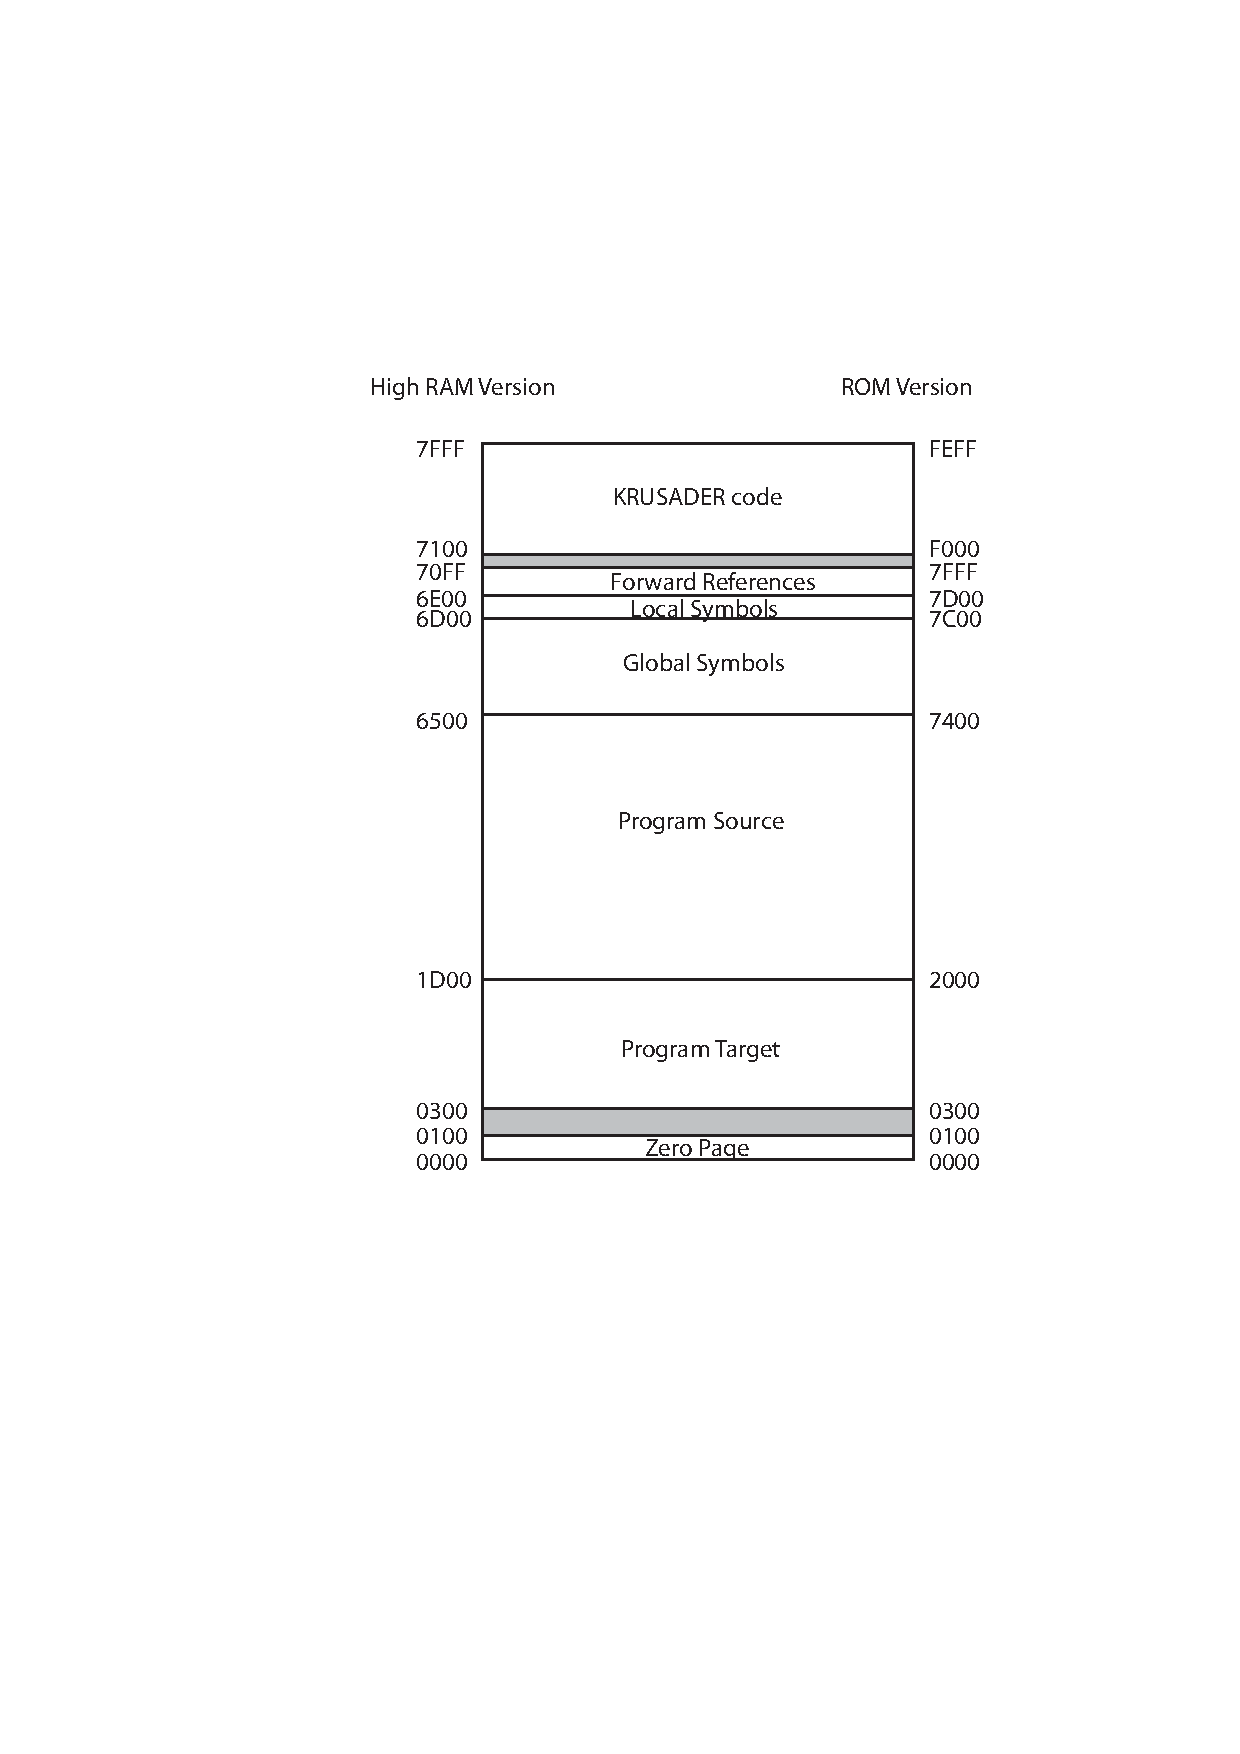
\includegraphics[scale=0.85]{Memory.pdf}
\caption{Memory map for both the high RAM and the ROM versions of \krusader.
Note that the global symbol table starts at the local/global table boundary and grows downwards, whereas the 
program source starts at the low address and grows upwards.
As mentioned in section \protect\ref{sec:memory}, the important values are the high byte of the target
memory, the high byte of the local/global symbol table boundary, and the start of the source code storage.  For the RAM version, the values are \texttt{\$03, \$6D, \$00} and \texttt{\$1D}, and for the ROM version
they are \texttt{\$03, \$7C, \$00} and \texttt{\$20}.
After initialisation, these values are stored in zero page locations \texttt{\$F8, \$F9, \$FE} and \texttt{\$FF}.
}
\label{fig:memmap}
\end{figure}

\krusader also
uses a number of zero page locations, but mostly as an input buffer and during assembly.  The only
locations that must be maintained are \texttt{\$F8, \$F9, \$FE} and \texttt{\$FF}.  These hold
the high byte of the default assembled code storage location, the high byte of the local/global
symbol table boundary, and the low and high bytes of the source code storage location respectively
(See figure \ref{fig:memmap} for the appropriate values).
Replica 1 users need to beware of BASIC because it may overwrite these four values, so they need to 
be restored before returning to the \krusader shell\footnote{The \replica{P} command is useful 
for restoring the default values to these zero page memory locations.}.  

\subsubsection{Changing Default Memory Locations}
\label{sec:mem_defaults}
For the RAM based version of \krusader, the default values can be altered by changing the values at memory locations \texttt{\$7101}, \texttt{\$7105} and \texttt{\$7109} in the assembler code.
For the ROM based version, the default values can only be altered after the program has been run, and the alternative values must be entered directly into the zero page locations mentioned above, before resuming \krusader at location 
\texttt{\$F01A}\footnote{The \replica{P} command will overwrite any values entered in this way.}.

\subsection{Source Tokenisation Scheme}
\label{sec:token}

Any entered source is stored in a tokenised form in order to save space.  The tokenisation
employed is quite simple because there was even less space available in the code to implement it!
Three special codes are employed -- \texttt{\$01} as a field terminator, 
\texttt{\$00} as a line terminator, and \texttt{\$02 00} to indicate a blank line.
Labels, arguments and comments are stored as entered with the field terminator marking their end, 
and mnemonics and directives are encoded as a single byte.  Program end is indicated by a line
starting with \texttt{\$00}.  
This simple scheme results in a reduction of the source code size by a factor of 2 to 3.

Also provided in the \krusader distribution is C source code for a program that can
convert more general source code formats to the required tokenised form, so that they
may be uploaded to the assembler.  However, this simple program does not translate
different formats for directives or addressing mode specification, so if any
such changes are required, they must be done manually. 
Once you have the converted source data, simply 
launch \krusader as normal, enter the monitor and load in the tokenised data to the
source storage memory, and resume.  The source will then be available to \krusader
as if you had typed it in as normal.  However, syntax and formatting errors in the source may not be well handled
since the error handling is designed around the restrictions placed on source input in the
usual manner.

One useful thing to keep in mind is the \replica{N} command simply clears the source program
from memory by putting a \texttt{\$00} as the very first byte of the source storage location.
So if \replica{N} is typed accidentally, the source can be easily restored.  To do this manually, simply enter
the monitor using \replica{\$}, and change this initial byte to either \texttt{\$01} if there was no
label, or the first byte of the label, and then resume \krusader as normal with \texttt{711AR(F01AR)}.
This process is automated by the \replica{P} command.
You should note however that there is no way to recover source lines deleted with the
\replica{X} or \replica{E} commands since the memory is immediately overwritten.

\subsection{Moving Memory}

If you want to copy a block of memory to another location (if you are backing up source 
or machine code via the expansion interface for example), you can make use of one
of the memory moving subroutines inside the assembler as follows.  First work out non-overlapping source
and destination addresses -- call these \replica{srcL, srcH, destL} and \replica{destH}, and then
the size of memory to move -- \replica{sizeL} and \replica{sizeH}.  
(You can do this using the \replica{M} command for 
source or watching the output of the \replica{A} command for assembled code.)  Then drop into the 
monitor using the \replica{\$} command, and enter:
\replica{50: srcL srcH destL destH sizeL sizeH}
to set the parameters, and \replica{7322R} (\replica{F222R}) to do the move.

\subsection{Testing}

\krusader comes with a number of sample programs, both in binary and hex dump formats,
and these are useful for verifying its correct operation.  The most important sample in this regard
is \texttt{TestSuite.asm}, which contains a number of modules for testing the
assembler.  (For the 65C02 version, there is instead the pair of source files
\texttt{TestSuiteC.asm} for the pure 6502 tests, and \texttt{TestSuite65C02.asm} for tests of the 65C02 extensions.)
The first test of course is that the source assembles without error, 
then \replica{R MAIN} will cause the program to verify its own assembled code and report any errors.
This test suite covers all the 6502 instructions, using all their addressing 
modes and a couple of different formats for arguments where relevant, as well as 
each of the available directives.  
In addition, both forward referencing and the various kinds of expressions 
supported by \krusader are tested -- both alone and in combination with various addressing modes.  A successful run of this suite of tests is a very good indication that \krusader
is functioning properly.

Because of the size of the test suite code, it can not be run with the RAM version
of \krusader without changing the start address for program source storage as
described in section \ref{sec:mem_defaults} above in order
to allow enough room for the source code, the assembled code, and the global symbol table.
Specifically, prior to running \krusader, the value at address \texttt{\$7101} needs to be changed to \texttt{\$14}, or if \krusader is already running, this value of \texttt{\$14} 
can be loaded directly into the zero page address \texttt{\$FF}.

%\subsection{Version Information}

%As mentioned in the introduction, \krusader was primarily designed to fit in the Replica 1 ROM
%in the range \replica{F000-FEFF}.  This places quite a strong constraints on its size, and one 
%consequence of this is that there is no room for a command purely to report version 
%information.  Instead, the last two bytes of the \krusader object code contain this %information,
%with the major version number at \replica{7FFE} (\replica{FEFE}), and the minor version number
%at \replica{7EFF} (\replica{FEFF}).

	
\section{Release History}
\label{sec:history}

\begin{itemize}
	\item \krusader 1.0 (May 2006)
		\begin{itemize}
			\item First version released
			\item Target CPU is 6502 only
			\item Buggy
		\end{itemize}
	\item \krusader 1.1 (July 2006)
		\begin{itemize}
			\item Fully tested version
			\item Comes with code for a thorough automated testing of itself
			\item Various enhancements over version 1, most notably:
			\begin{itemize}
				\item Forward references can cross module boundaries
				\item Symbol redefinition is reported as an error
				\item comment only lines
				\item Approximately 20\% faster assembly
			\end{itemize}
			\item This version was added to the Replica 1 SE ROM
		\end{itemize}
	\item \krusader 1.2 (August 2006)
		\begin{itemize}
			\item Functionally equivalent to version 1.1
			\item Fixes an obscure bug in version 1.1 that prevented assembly of \texttt{JMP}
				or \texttt{JSR} commands targetting page zero
			\item More compact implementation in places means implemented in approximately 100 fewer bytes than version 1.1
			\item Recommended for people who wish to extend Krusader by adding custom commands etc
		\end{itemize}
	\item \krusader 1.3 (August 2006)
		\begin{itemize}
			\item 65C02 commands fully supported by both the assembler and disassembler
			\item Better syntax checking than earlier versions
			\item Still fits inside the 3980 free bytes of the Replica 1 ROM!
		\end{itemize}
\end{itemize}

\end{document}
